\documentclass[review]{elsarticle}
%DIF LATEXDIFF DIFFERENCE FILE
%DIF DEL usixeOLD.tex   Wed Feb 27 09:15:32 2019
%DIF ADD usixe.tex      Wed May 29 14:06:08 2019
\usepackage{hyperref}
\usepackage[margin=1in]{geometry}
\usepackage{graphicx}
\usepackage{amsmath}
\usepackage{placeins}
\usepackage{comment}
\usepackage{fancyref}
\usepackage{color}
%\usepackage{cite}

\def\bibsection{\section*{References}}

\journal{Journal of Nuclear Materials}
\bibliographystyle{elsarticle-num}
%DIF PREAMBLE EXTENSION ADDED BY LATEXDIFF
%DIF CTRADITIONAL PREAMBLE %DIF PREAMBLE
\RequirePackage{color}\definecolor{RED}{rgb}{1,0,0}\definecolor{BLUE}{rgb}{0,0,1} %DIF PREAMBLE
\RequirePackage[stable]{footmisc} %DIF PREAMBLE
\DeclareOldFontCommand{\sf}{\normalfont\sffamily}{\mathsf} %DIF PREAMBLE
\providecommand{\DIFaddtex}[1]{{\protect\color{blue} \sf #1}} %DIF PREAMBLE
\providecommand{\DIFdeltex}[1]{{\protect\color{red} [..\footnote{removed: #1} ]}} %DIF PREAMBLE
%DIF SAFE PREAMBLE %DIF PREAMBLE
\providecommand{\DIFaddbegin}{} %DIF PREAMBLE
\providecommand{\DIFaddend}{} %DIF PREAMBLE
\providecommand{\DIFdelbegin}{} %DIF PREAMBLE
\providecommand{\DIFdelend}{} %DIF PREAMBLE
%DIF FLOATSAFE PREAMBLE %DIF PREAMBLE
\providecommand{\DIFaddFL}[1]{\DIFadd{#1}} %DIF PREAMBLE
\providecommand{\DIFdelFL}[1]{\DIFdel{#1}} %DIF PREAMBLE
\providecommand{\DIFaddbeginFL}{} %DIF PREAMBLE
\providecommand{\DIFaddendFL}{} %DIF PREAMBLE
\providecommand{\DIFdelbeginFL}{} %DIF PREAMBLE
\providecommand{\DIFdelendFL}{} %DIF PREAMBLE
%DIF HYPERREF PREAMBLE %DIF PREAMBLE
\providecommand{\DIFadd}[1]{\texorpdfstring{\DIFaddtex{#1}}{#1}} %DIF PREAMBLE
\providecommand{\DIFdel}[1]{\texorpdfstring{\DIFdeltex{#1}}{}} %DIF PREAMBLE
\newcommand{\DIFscaledelfig}{0.5}
%DIF HIGHLIGHTGRAPHICS PREAMBLE %DIF PREAMBLE
\RequirePackage{settobox} %DIF PREAMBLE
\RequirePackage{letltxmacro} %DIF PREAMBLE
\newsavebox{\DIFdelgraphicsbox} %DIF PREAMBLE
\newlength{\DIFdelgraphicswidth} %DIF PREAMBLE
\newlength{\DIFdelgraphicsheight} %DIF PREAMBLE
% store original definition of \includegraphics %DIF PREAMBLE
\LetLtxMacro{\DIFOincludegraphics}{\includegraphics} %DIF PREAMBLE
\newcommand{\DIFaddincludegraphics}[2][]{{\color{blue}\fbox{\DIFOincludegraphics[#1]{#2}}}} %DIF PREAMBLE
\newcommand{\DIFdelincludegraphics}[2][]{% %DIF PREAMBLE
\sbox{\DIFdelgraphicsbox}{\DIFOincludegraphics[#1]{#2}}% %DIF PREAMBLE
\settoboxwidth{\DIFdelgraphicswidth}{\DIFdelgraphicsbox} %DIF PREAMBLE
\settoboxtotalheight{\DIFdelgraphicsheight}{\DIFdelgraphicsbox} %DIF PREAMBLE
\scalebox{\DIFscaledelfig}{% %DIF PREAMBLE
\parbox[b]{\DIFdelgraphicswidth}{\usebox{\DIFdelgraphicsbox}\\[-\baselineskip] \rule{\DIFdelgraphicswidth}{0em}}\llap{\resizebox{\DIFdelgraphicswidth}{\DIFdelgraphicsheight}{% %DIF PREAMBLE
\setlength{\unitlength}{\DIFdelgraphicswidth}% %DIF PREAMBLE
\begin{picture}(1,1)% %DIF PREAMBLE
\thicklines\linethickness{2pt} %DIF PREAMBLE
{\color[rgb]{1,0,0}\put(0,0){\framebox(1,1){}}}% %DIF PREAMBLE
{\color[rgb]{1,0,0}\put(0,0){\line( 1,1){1}}}% %DIF PREAMBLE
{\color[rgb]{1,0,0}\put(0,1){\line(1,-1){1}}}% %DIF PREAMBLE
\end{picture}% %DIF PREAMBLE
}\hspace*{3pt}}} %DIF PREAMBLE
} %DIF PREAMBLE
\LetLtxMacro{\DIFOaddbegin}{\DIFaddbegin} %DIF PREAMBLE
\LetLtxMacro{\DIFOaddend}{\DIFaddend} %DIF PREAMBLE
\LetLtxMacro{\DIFOdelbegin}{\DIFdelbegin} %DIF PREAMBLE
\LetLtxMacro{\DIFOdelend}{\DIFdelend} %DIF PREAMBLE
\DeclareRobustCommand{\DIFaddbegin}{\DIFOaddbegin \let\includegraphics\DIFaddincludegraphics} %DIF PREAMBLE
\DeclareRobustCommand{\DIFaddend}{\DIFOaddend \let\includegraphics\DIFOincludegraphics} %DIF PREAMBLE
\DeclareRobustCommand{\DIFdelbegin}{\DIFOdelbegin \let\includegraphics\DIFdelincludegraphics} %DIF PREAMBLE
\DeclareRobustCommand{\DIFdelend}{\DIFOaddend \let\includegraphics\DIFOincludegraphics} %DIF PREAMBLE
\LetLtxMacro{\DIFOaddbeginFL}{\DIFaddbeginFL} %DIF PREAMBLE
\LetLtxMacro{\DIFOaddendFL}{\DIFaddendFL} %DIF PREAMBLE
\LetLtxMacro{\DIFOdelbeginFL}{\DIFdelbeginFL} %DIF PREAMBLE
\LetLtxMacro{\DIFOdelendFL}{\DIFdelendFL} %DIF PREAMBLE
\DeclareRobustCommand{\DIFaddbeginFL}{\DIFOaddbeginFL \let\includegraphics\DIFaddincludegraphics} %DIF PREAMBLE
\DeclareRobustCommand{\DIFaddendFL}{\DIFOaddendFL \let\includegraphics\DIFOincludegraphics} %DIF PREAMBLE
\DeclareRobustCommand{\DIFdelbeginFL}{\DIFOdelbeginFL \let\includegraphics\DIFdelincludegraphics} %DIF PREAMBLE
\DeclareRobustCommand{\DIFdelendFL}{\DIFOaddendFL \let\includegraphics\DIFOincludegraphics} %DIF PREAMBLE
%DIF END PREAMBLE EXTENSION ADDED BY LATEXDIFF

\begin{document}
\begin{frontmatter}
\title{A molecular dynamics study of the behavior of Xe in U$_{3}$Si$_{2}$}

\author[inl]{Benjamin Beeler\corref{qwe}}
\cortext[qwe]{Corresponding author}
\ead{benjamin.beeler@inl.gov}
\author[lanl]{David Andersson}
\author[lanl]{Michael WD Cooper}
\author[inl]{Yongfeng Zhang}
\address[inl]{Idaho National Laboratory, Idaho Falls, ID 83415}
\address[lanl]{Los Alamos National Laboratory, Los Alamos, NM 87545}



\begin{abstract}

Uranium-silicide (U-Si) fuels are being pursued as a possible accident tolerant fuel (ATF). This uranium alloy fuel benefits from higher thermal conductivity and higher fissile density compared to uranium dioxide (UO$_{2}$). The role of fission gas swelling on the operational performance of U-Si fuels remains an open question, however, fission gas swelling is a critical phenomenon in UO$_{2}$, U-Zr and U-Mo nuclear fuels. Given the lack of experimental data, in order to study the fundamentals of bubble formation and evolution in U-Si, it is critical that there be an atomistic description of Xe within the U-Si system. In this work, a recently developed U-Si MEAM interatomic potential is leveraged to generate a description of the U-Si-Xe system fit to density functional theory data. The point defect energies of Xe in U$_{3}$Si$_{2}$ are determined, in addition to the point defect segregation energy for Xe with respect to two grain boundary orientations. Finally, the properties of small Xe bubbles are analyzed and an equation of state is developed. 

\end{abstract}
\end{frontmatter}

\section{Introduction}

Accident-tolerant fuel (ATF) \cite{zinkle2014} is being considered for future and existing light-water reactors (LWRs). ATFs aim to provide additional coping time in the event of an accident (such as a loss of coolant accident) due to the inherent properties of the fuel, while maintaining good operational characteristics. Uranium-silicide (U-Si), and particularly U$_{3}$Si$_{2}$, is a fuel candidate for ATFs. U$_{3}$Si$_{2}$ exhibits higher uranium density than traditional UO$_{2}$ LWR fuel, thus allowing for the possibility of reduced enrichments, fewer assemblies and/or an extended lifetime in the core. U$_{3}$Si$_{2}$ also possesses a higher thermal conductivity than UO$_{2}$, allowing for a lower fuel centerline temperature and more efficient heat removal during off-normal conditions. As such, extensive experimental and computational investigation has been undertaken within the past few years studying thermophysical properties \cite{white2015}, irradiation behavior \cite{carmack2015, miao2017a, miao2018}, fabrication \cite{harp2015}, fuel-clad chemical interaction \cite{he2017} point defects \cite{middleburgh2016} and empirical models of gaseous swelling \cite{miao2017, miao2018a}. 

One prevalent area of investigation in U-Si fuels is the nature, and extent, of swelling during reactor operation. Historical studies \cite{shimizu1965} focused on the irradiation behavior of U$_3$Si$_2$ and showed substantial swelling ($>$5\%). Recently, ion implantation experiments and multiscale modeling have been employed to investigate fission gas behavior in U$_3$Si$_2$ in an attempt to better understand (and hopefully predict) the mechanisms of gaseous swelling. Ion irradiations \cite{miao2017a, miao2018, yao2018} have been performed to study bubble formation and morphology over a range of temperatures. These studies provide valuable information on high fission density and high fission rate and especially inform the amorphization and recrystallization behavior of these fuels. Rate theory has also been utilized \cite{miao2017, miao2018a} to study normal and off-normal fission gas behavior in light water reactors. These models can be parametrized to correspond to existing experimental data and then applied to a variety of operational scenarios to predict fuel swelling behavior. The predicted swelling behavior in these models has been shown to be very sensitive to a variety of key parameters \cite{miao2017}. Recently, a phase-field model has been developed to describe fission gas swelling in U$_{3}$Si$_{2}$ \cite{fy17usi, fy18usi} that is capable of describing both intra- and inter-granular bubbles in a polycrystalline microstructure. The phase-field model was parameterized based on density functional theory (DFT) calculations and molecular dynamics simulations. This model was also shown to be sensitive to a variety of parameters (including Xe equation of state, surface energies, and diffusion coefficients) in addition to including a number of assumptions. Thus, the procurement of accurate properties for U$_3$Si$_2$ is critical for the proper behavior of these various swelling models and the subsequent accurate prediction of fission gas swelling. 

First principles calculations on the U$_3$Si$_2$ system have been performed in order to more accurately inform mesoscale models \cite{noordhoek2016, middleburgh2016, andersson2018, chattaraj2018, wang2016} and a variety of properties including point defect formation energies, elastic constants and thermodynamic functions have been determined. These studies have provided critical data to increase the fidelity of mesoscale models of the U$_3$Si$_2$ system. For fundamental understanding of U$_3$Si$_2$ at non-zero temperatures, first principles methods cede to more semi-empirical descriptions of interatomic interactions. Such methods allow for the study of much larger and complex systems, including the ability to analyze systems with millions of atoms at high temperature, studying dynamics over nanosecond time scales, investigation of voids, clusters, diffusion, etc. The accuracy of these methods depends on the ability of an interatomic potential to describe physical properties. Recently, a modified embedded-atom method (MEAM) potential was published \cite{beelerusi} that describes the U-Si system, with a particular emphasis on the U$_3$Si$_2$ phase. However, there does not yet exist an interatomic potential capable of describing the U-Si-Xe ternary system. Such a ternary potential is required for the investigation of atomistic behavior of Xe segregation at interfaces, bubble formation, bubble growth and internal pressure, and irradiation enhanced diffusion. 

In this work, a semi-empirical modified embedded-atom method (MEAM) interatomic potential is developed for the investigation of Xe in U$_3$Si$_2$. The potential is utilized to investigate the segregation energy of Xe atoms at multiple grain boundaries in U$_3$Si$_2$. The nature of small Xe bubbles is also studied and an equation of state is developed that can describe Xe in bubbles in U$_3$Si$_2$. This is the first interatomic potential capable of describing the U-Si-Xe ternary system.

\section{Interatomic Potential Fitting Procedure}
The modified embedded-atom method theory has been well described elsewhere and will not be repeated in this manuscript \cite{baskes1997, baskes2000, baskes2014, baskes1989, valone2006, liu1999, lee2000, lee2001, lee2003}. 

In order to create a functional U-Si-Xe ternary interatomic potential, there must first exist (or be generated) suitable potentials for each individual element. For U, Si and the U-Si contributions, the recently developed interatomic potential from Beeler, et al. \cite{beelerusi} is utilized. This potential can accurately reproduce a variety of properties of U$_3$Si$_2$ at 0 K and elevated temperatures. This potential also shows reasonable accuracy in describing adjacent U-Si phases in the phase diagram (U$_3$Si and USi). The U-Si potential utilized a MEAM U potential from Moore, $\textit{et al.}$ \cite{moore2015}. The U MEAM potential performs excellently in describing the body-centered cubic phase of U and the alloy behavior of U-Zr. The description of Xe is taken from Beeler, et al. \cite{beelerASTM} which showed reasonable agreement of U-Xe theoretical intermetallic structures, and good agreement with density functional theory for Xe substitutional defects in $\gamma$U. 

The fitting procedure to develop cross-species parameters (U-Xe and Si-Xe interactions) involves a reference phase (chosen to be B1-UXe and B1-SiXe) and a starting guess for MEAM parameters. The reference phase provides a crystal structure and cohesive energy to serve as a basis for an energetic relationship between two species and need not be an equilibrium phase. MEAM parameter refinement is subsequently performed via a script that provides a random change to all relevant MEAM parameters. This updated potential is then input into LAMMPS \cite{plimpton1995} and a series of simulations are performed, the output of which is utilized to calculate a weighted-error summation. The script then either accepts or rejects the prescribed changes to the MEAM parameters based on the reduction of the total weighted-error. The emphasis of the fitting procedure was on point defect properties of Xe in U$_{3}$Si$_{2}$, attempting to fit to DFT-based incorporation energies \cite{andersson2018}. The Xe substitutional energy on each of the three lattice sites (2a-U1, 4h-U2, 4g-Si) and the Xe interstitial energy were included as the fitting targets. The pure Xe interatomic potential was held fixed, and only the U-Xe and Si-Xe cross-species MEAM parameters were allowed to evolve. The starting guess for both U-Xe and Si-Xe cross species terms is taken from the U-Xe desription from \cite{beelerASTM}. It should be noted that additionally the reference phase energy and lattice constant were allowed to evolve for both the U-Xe B1 and Si-Xe B1 structures.

The energy landscape of U$_3$Si$_2$ is very complex, and the point defect properties are reasonably accurate, but still show significant variance from DFT. The MEAM vacancy formation energy data from Beeler, et al. \cite{beelerusi} is reproduced here in table \ref{tab:defs} and compared to the DFT data from Middleburgh, et al. \cite{middleburgh2016}. To ensure that the lowest energy configurations were obtained in the course of the fitting procedure, the U$_3$Si$_2$ system with a Xe defect is initialized at 1500 K and slowly quenched to 0 K over 50 ps with a 1 fs timestep, in order to allow for the reorientation of the Xe defect into the lowest energy configuration. The subsequent incorporation energy is then determined, utilizing equation \ref{eq:eincorp}. 

\begin{table}[h!]
\caption{Properties of point defects in U$_{3}$Si$_{2}$ at 0 K. Results from the MEAM U-Si potential are compared to DFT calculations \cite{middleburgh2016}. Units in eV.}\label{tab:defs}
\begin{center}
\begin{tabular}{|c|c|c|}
 \hline
 & DFT & U-Si MEAM \\
 \hline
 U1 vac & 0.68 & 1.16 \\
 U2 vac & 1.20 & 1.25 \\
 Si vac & 1.59 & 1.70 \\
 \hline
\end{tabular}
\end{center}
\label{default}
\end{table}%

The incorporation energy is defined as the energy associated with placing a Xe atom into a trap site:

\begin{equation}
\label{eq:eincorp}
E_{inc} = E^{*Xe} - E^*
\end{equation}

where E$^{*Xe}$ is the energy of the supercell with a Xe defect and E$^*$ is the energy of the supercell with the specific trap site. The trap site energy for the Xe interstitial is simply the supercell energy with no defects present. This is an identical definition to the incorporation energy described by Andersson \cite{andersson2018}, albeit in a modified formulation. The resultant interatomic potential is provided in table \ref{tab:lib} for each elemental species and table \ref{tab:meam} for the cross species parameters. Screening parameters are given in LAMMPS format (i.e., C$_{max}$(I,J,K) is a screening parameter when I-J pair is screened by K, where I, J and K are atom types). Readers can refer to the LAMMPS \cite{plimpton1995} documentation for full implementation of these parameters. \DIFaddbegin \DIFadd{The pair-potential for the U-Si, U-Xe and Si-Xe interactions are shown in Fig. \ref{fig:dimer} for reference.
}\DIFaddend 

\begin{table}[h]
\caption{Si, U and Xe MEAM potential parameters. }\label{tab:lib}
\begin{center}
\begin{tabular}{|c|c|c|c|}
 \hline
 Parameter & Si-MEAM \cite{beelerusi} & U-MEAM \cite{moore2015} & Xe-MEAM \cite{beelerASTM} \\
 \hline
 attrac & -0.2073 & 0.105 & 0 \\
 repuls & -0.1876 & 0.105 & 0 \\
 alpha & 5.5576 & 5.1 & 7.8 \\
 $\beta$$^{0}$ & 4.0501 & 4.8 & 4.9 \\
 $\beta$$^{1}$ & 5.6911 & 6 & 0 \\
 $\beta$$^{2}$ & 4.5856 & 6 & 0 \\ 
 $\beta$$^{3}$ & 5.5305 & 6 & 0 \\
 alat (\AA) & 5.431 & 4.28 & 6.93 \\
 E$_{c}$ (eV) & 4.63 & 5.27 & 0.032 \\
 A & 0.829 & 0.98 & 0\\
 t$^{0}$ & 1 & 1 & 1 \\
 t$^{1}$ & 2.0601 & 2.5 & 1 \\
 t$^{2}$ & 4.6769 & 4.0 & 1\\
 t$^{3}$ & -1.3216 & 1.2 & 1 \\
 C$_{min}$ & 0.9666 & 1.0 & 2.0 \\ 
 C$_{max}$ & 2.7994 & 1.9 & 2.8 \\
 rho & 1.0 & 1.0727 & 0.154 \\
 \hline
\end{tabular}
\end{center}
\label{default}
\end{table}%


\begin{table}[h]
\caption{U-Si, U-Xe and Si-Xe MEAM potential parameters. For alpha and screening parameters (C$_{min/max}$), i and j refer to the species labeled in the header. For example: for U-Xe, i=U, j=Xe. }\label{tab:meam}
\begin{center}
\begin{tabular}{|c|c|c|c|}
 \hline
 Parameter & U-Si MEAM \cite{beelerusi} & U-Xe MEAM & Si-Xe MEAM \\
 \hline
 E$_{c}$ (eV) & 5.36 & 0.644 & 0.743 \\ 
 r$_{e}$ (\AA) & 3.05 & 3.132 & 3.447 \\
 lattce & l12 & b1 & b1\\
 r$_{c}$ (\AA) & 6.0 & 6.0 & 6.0\\
 attrac & -0.1129 & -0.067 & 0.062 \\
 repuls & 0.2171 & 0.148 & -0.091 \\
 alpha(i,j) & 4.793 & 7.817 & 5.393 \\
 C$_{min}$(i,i,j) & 0.985 &1.22 & 1.58\\
 C$_{max}$(i,i,j) & 2.313 & 2.65 & 2.75\\
 C$_{min}$(i,j,i) & 0.385 & 1.78 & 2.2 \\
 C$_{max}$(i,j,i) & 1.974 & 2.44 & 2.59\\
 C$_{min}$(i,j,j) & 0.926 & 2.0 & 2.0\\
 C$_{max}$(i,j,j) & 2.718 & 2.8 & 2.8\\
 C$_{min}$(j,j,i) & 1.175 & 2.0 & 2.0\\ 
 C$_{max}$(j,j,i) & 1.435 & 2.8 & 2.8 \\
 \hline
\end{tabular}
\end{center}
\label{default}
\end{table}%

\DIFaddbegin \begin{figure}[hbt]
	\centering
	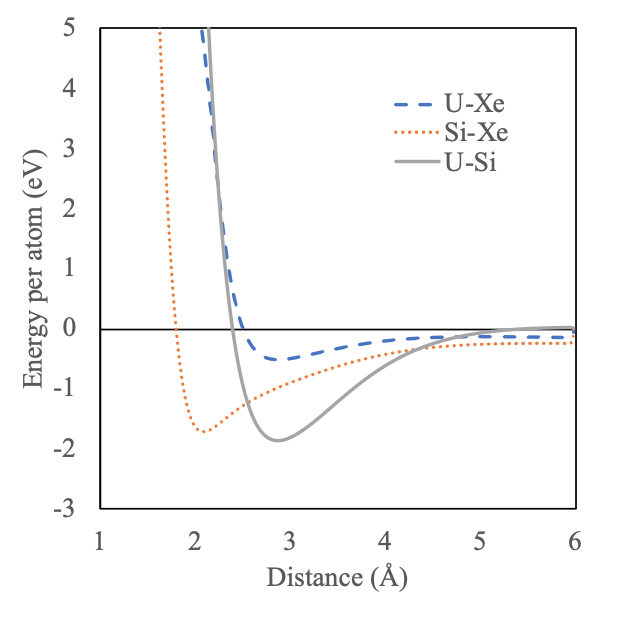
\includegraphics[width=0.7\textwidth]{dimer_E.png}
 \caption{ \DIFaddFL{The pair potential for the U-Si, U-Xe and Si-Xe interactions. The energy per atom (in eV) is shown as a function of distance (in \AA). }}\label{fig:dimer}
\end{figure}

\DIFaddend \FloatBarrier

LAMMPS MEAM-specific parameters are identical to those outlined by Beeler \cite{beelerusi}. It should also be noted that a non-standard implementation of MEAM within LAMMPS (which relates to modification of the smooth cutoff function) was utilized for the existing U MEAM potential and the subsequent U-Si potentials. Please contact the authors to obtain the required modifications in order to accurately utilize the potential. 

The resultant Xe defect incorporation energies are shown in table \ref{tab:xeinc} for all three atomic sites (2a-U1, 4h-U2, 4g-Si) and a Xe interstitial. \DIFaddbegin \DIFadd{These three atomic sites are shown in Fig. \ref{fig:defect_sites}. }\DIFaddend There is not perfect agreement between the MEAM potential and the DFT calculations, as one could expect from the inherent deviations in self-defect formation energies in U$_3$Si$_2$. However, reasonable agreement is observed both on the absolute magnitude of the various defect incorporation energies and the relative magnitude of the incorporation energies comparing the interstitial to substitutionals. The MEAM potential does show a preference for forming U2 Xe substitutionals, which is not present within the DFT study. However, the Xe interstitial is substantially the highest in incorporation energy. This is considered reasonable, albeit imperfect, agreement. 

\DIFaddbegin \begin{figure}[hbt]
	\centering
	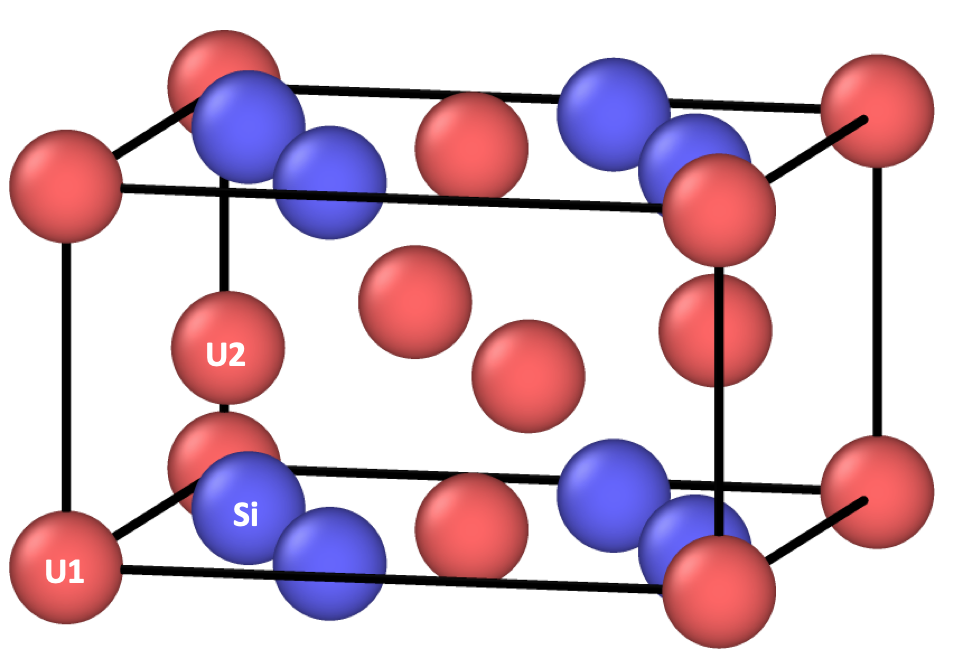
\includegraphics[width=0.7\textwidth]{defect_sites.png}
 \caption{ \DIFaddFL{The U$_3$Si$_2$ unit cell with the three unique substitutional sites denoted U1 (2a), U2 (4h) and Si (4g). Red atoms are U and blue atoms are Si. }}\label{fig:defect_sites}
\end{figure}

\DIFaddend \begin{table}[h]
\caption{Incorporation energy of Xe defects in U$_3$Si$_2$. Results from the MEAM interatomic potential are compared to DFT calculations \cite{andersson2018}. }\label{tab:xeinc}
\begin{center}
\begin{tabular}{|c|c|c|c|}
 \hline
 & DFT & U-Si-Xe MEAM \\
 \hline
 Xe int & 5.36 & 4.53 \\ 
 Xe sub U1 & 3.60 & 3.91 \\ 
 Xe sub U2 & 3.57 & 2.93 \\ 
 Xe sub Si & 3.45 & 3.90 \\ 
 \hline
\end{tabular}
\end{center}
\label{default}
\end{table}%

\FloatBarrier

\section{Verification of the U-Si-Xe interatomic potential}

The comparison of the equation of state (EOS) for Xe was first established to ensure the validity of the existing Xe potential and its correct implementation within LAMMPS. The pressure as a function of specific volume is shown in Fig. \ref{fig:xe_eos} compared to the EOS as calculated by Ronchi \cite{ronchi1981} at 400 K, 600 K, 800 K, 1000 K and 1200 K. Generally excellent agreement is observed. Minimal error is present for low pressure systems, although some error does exist once systems reach very high pressures (above 1 GPa). The MEAM potential tends to show a slightly higher pressure for low temperature systems, but this error diminishes at the higher temperatures investigated. The root-mean squared deviation (RMSD) over the entire data set is 195 MPa (note that the maximum pressure in the dataset is 3.2 GPa). Since the range of pressures in this dataset covers multiple orders of magnitude, it can be better to investigate error with a normalized RMSD (NRMSD). One way of constructing a NRMSD is by dividing the RMSD by the range (the difference of the maximum and minimum) of the dataset. In this way, the NRMSD of the MEAM EOS compared to the Ronchi EOS is 6\%. This is acceptable, if imperfect, agreement with data in the literature and satisfactorily shows the suitability of the Xe MEAM potential formalism and implementation. \DIFaddbegin \DIFadd{The Xe radial distribution has also been analyzed as a function of density. Xe at high pressures and temperatures retain a gas-like radial distribution function, while Xe at high pressures and low temperatures close to the critical point (290 K) begin to exhibit a liquid-like radial distribution function. This generally corresponds to what is expected from the phase diagram \cite{cook1961}.
}\DIFaddend 

\begin{figure}[hbt]
	\centering
	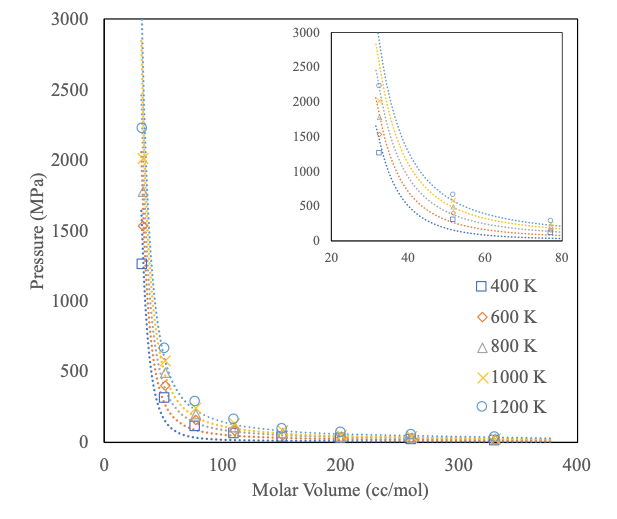
\includegraphics[width=0.7\textwidth]{Xe_T_PvsV.png}
 \caption{Pressure as a function of specific volume for the Xe MEAM potential and the EOS as determined by Ronchi \cite{ronchi1981} at five temperatures. Ronchi data is included as dashed lines, while the data from the MEAM potential is denoted by the symbols in the legend at the same temperatures. \DIFaddbeginFL \DIFaddFL{An inset is included for high pressure/density data.}\DIFaddendFL }\label{fig:xe_eos}
\end{figure}

\FloatBarrier

A further test of the potential is comparing formation energies and lattice constants of U-Xe and Si-Xe compounds. As no such compounds exist experimentally, they must be simulated. Density functional theory (DFT) calculations were performed on theoretical intermetallic phases of U-Xe and Si-Xe, neglecting Van der Waals interactions. Systems are investigated using the Vienna $\textit{ab initio}$ Simulation Package (VASP) \cite{vasp1, vasp2, vasp3, vasp4}. The projector augmented wave (PAW) method \cite{paw1, paw2} is utilized within density functional theory \cite{dft1, dft2}. Calculations are performed using the Perdew-Burke-Ernzerhof (PBE) \cite{pbe1, pbe2} generalized gradient approximation (GGA) for the description of the exchange-correlation. Methfessel and Paxton's smearing method \cite{methfessel} of the first order is used with a width of 0.1 eV to determine partial occupancies for each wavefunction. Wavefunction optimization was truncated when the energy difference was less than 10$^{-4}$ eV. The optimization procedure was truncated when the residual forces for the relaxed atoms were less than 0.01 eV/{\AA}. The energy cutoff is increased to 500 eV and symmetry is switched off for all calculations. A support grid is utilized for the evaluation of augmentation charges. A single unit cell was utilized for each of the L1$_2$, B1 and B2 intermetallic structures for both U-Xe and Si-Xe systems and progressively more dense kpoint meshes were utilized until the energy of the system varied by less than 5 meV. 

The formation energies and lattice constants of three theoretical intermetallic structures for the U-Xe and Si-Xe systems are shown in table \ref{tab:inter}, comparing the DFT calculations to the results from the interatomic potential. Although the reference phases are the B1 U-Xe and B1 Si-Xe, the equilibrium energies and volumes were allowed to change throughout the fitting process, and thus none of the structures in Table \ref{tab:inter} were included as fitting targets. This comparison serves as a test of the applicability of the cross-species interatomic potentials. Reasonable quantitative agreement is observed for most intermetallic structures. The B1 structures show generally lower formation energies compared to DFT but variance of less than 3\% in the equilibrium lattice constant. However, the ratio of the formation energies for B1 U-Xe/Si-Xe shows considerable agreement, where the B1 U-Xe/Si-Xe formation energy ratio for the DFT calculations is 0.78, the ratio for the MEAM potential is 0.79. For the U$_3$Xe L1$_2$ structure, impressive accuracy is observed for both formation energy and equilibrium lattice constant. For the Si$_3$Xe, the formation energy is substantially overestimated and the volume per atom is underestimated. This is somewhat consistent with the behavior of the original U-Si potential, which performs more poorly for Si-rich phases. Finally for the B2 crystal structure, the lattice constant for the UXe system and the formation energy for the SiXe system show excellent agreement. However, the formation energy for the UXe system and the lattice constant for the SiXe system show considerable disagreement. In summary, there is not perfect agreement of the results from the MEAM potential compared to DFT calculations for this set of theoretical intermetallic phases. However, given that none of these systems were directly included in the fitting and that the systems of interest will typically be U-rich and Xe-dilute, the overall performance of the potential is considered quite good. 

%Additionally, both a U-Xe and Si-Xe dimer were simulated and the formation energy and dimer distance are reported in table \ref{tab:inter}.

\begin{table}[h]
\caption{Formation energies (E$_f$) and equilibrium lattice constants (a$_0$) of theoretical intermetallic structures of U-Xe and Si-Xe. Results from the MEAM interatomic potential are compared to DFT calculations. }\label{tab:inter}
\begin{center}
\begin{tabular}{|c|cc|cc|}
 \hline
 & \multicolumn{2}{c|}{U-Si-Xe MEAM} & \multicolumn{2}{c|}{DFT} \\
 \hline
 & a$_0$ (\AA) & E$_f$ (eV) & a$_0$ (\AA) & E$_f$ (eV) \\ 
 \hline
 U$_3$Xe L1$_2$ & 4.521 & 1.598 & 4.502 & 1.663 \\ 
 Si$_3$Xe L1$_2$ & 4.244 & 3.440 & 4.516 & 1.896 \\ 
 UXe B2 & 3.768 & 1.990 & 3.848 & 2.885 \\ 
 SiXe B2 & 5.080 & 2.114 & 4.102 & 2.122 \\ 
 UXe B1 & 6.264 & 2.007 & 6.087 & 2.938 \\ 
 SiXe B1 & 6.894 & 1.588 & 6.906 & 2.278 \\ 
% UXe Dimer & 2.879 & 2.131 & - & - \\
% SiXe Dimer & 2.094 & 0.602 & - & - \\
 \hline
\end{tabular}
\end{center}
\label{default}
\end{table}%

\FloatBarrier

\section{Results}

\subsection{Xe segregation at grain boundaries}

The grain boundary energies for U$_3$Si$_2$ systems have been previously determined \cite{beeler_usi_gb} and the suitability of the U-Si-Xe ternary interatomic potential has been established above. The grain boundary segregation energies are defined as 

\begin{equation}
\label{eq:eseg}
E_{seg} = E^{def}(r) - E^{def}(bulk) 
\end{equation}

where E$^{def}$(r) is the energy of the system with a Xe defect a distance \textit{r} from the grain boundary and E$^{def}$(bulk) is the energy of a system with a Xe defect in the bulk, in this work the bulk is defined as 30 {\AA} from the grain boundary. Three types of Xe defects are investigated: Xe interstitial, Xe substitutional on U lattice site and a Xe substitutional on Si lattice site. The segregation energy is determined at three unique temperatures: 400 K, 800 K and 1200 K. Two unique grain boundary planes are investigated, the (210) symmetric tilt and the (730) symmetric tilt, with respect to the (100) plane. These two directions were chosen because the (210) is a low energy grain boundary and the (730) is a high energy grain boundary \DIFdelbegin \DIFdel{\cite{beeler_usi_gb}}\DIFdelend \DIFaddbegin \DIFadd{(0.54 J/m$^2$ and 0.97 J/m$^2$, respectively \cite{beeler_usi_gb})}\DIFaddend . The simulation supercell consists of 4800 atoms for the (210) and 6960 atoms for the (730) grain boundary plane. Eighty unique simulations (for each temperature, defect type, grain boundary orientation and distance from the grain boundary) are performed in order to gain appropriate statistics, resulting in a total of 12,960 simulations in order to determine the segregation energies reported in this manuscript.

It was found that there were statistically insignificant differences in the segregation energy as a function of temperature, similar to the findings of self-defect segregation energies in U$_3$Si$_2$ \cite{beeler_usi_gb}. As such, the segregation energy for each defect as a function of distance can be averaged over all temperatures to obtain the general interaction of defects with the grain boundary. This was done for all three defect types near the (210) and (730) symmetric tilt grain boundaries and is displayed in Fig. \ref{fig:xeseg}. In Fig. \ref{fig:xeseg}, a clear negative segregation energy is present for all defect types within the first 5 {\AA} around the grain boundary. This segregation energy diminishes for all defect types once the defect distance becomes greater than 5 {\AA}. Beyond 5 {\AA}, the segregation energy oscillates around 0 eV, indicating no interaction of the defect with the grain boundary. Variation is present due to the inherent statistical uncertainty in the simulations. The average standard deviation for a given data point in Fig. \ref{fig:xeseg} is 0.3 eV.

Comparing grain boundary types, the (730) grain boundary plane typically shows lower segregation energies than the (210) grain boundary plane. It should be noted that the (730) grain boundary plane has a higher energy than the (210) plane. This shows that the higher energy grain boundary has a stronger preference for attracting and incorporating Xe defects. Comparing defect types, generally the Xe residing on a Si site exhibits the lowest segregation energy (strongest attraction) for the (210) grain boundary, while the Xe interstitial has the lowest segregation energy for the (730) grain boundary. For the (730) grain boundary, both Xe substitutional types exhibit similar segregation energies. 

\begin{figure}[hbt]
	\centering
	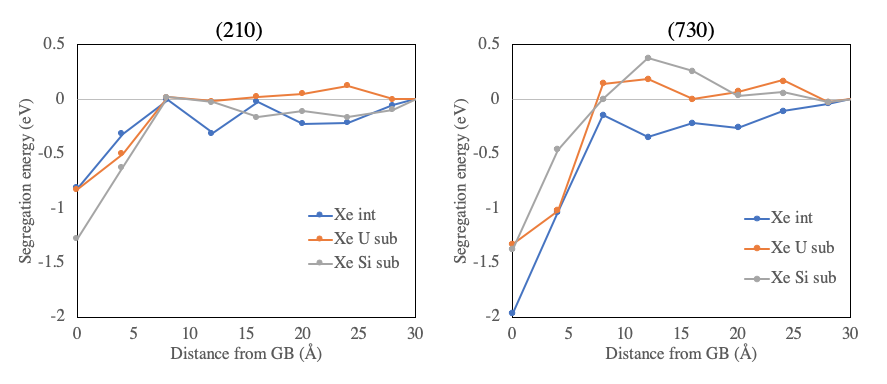
\includegraphics[width=0.9\textwidth]{Xe_Eseg.png}
 \caption{The average Xe defect segregation energies for three defect types at a (210) and a (730) symmetric tilt grain boundary.}\label{fig:xeseg}
\end{figure}

\FloatBarrier

This information can be utilized to parametrize sink strength models that affect Xe concentration evolution within mesoscale modeling methodologies \cite{was2007}.

\subsection{Properties of Xe bubbles in U$_3$Si$_2$}

Simulations are performed in an NVT ensemble to mimic a bubble in a very large system that effectively exerts a resistive pressure. This allows for the calculation of a Xe bubble pressure and a subsequent equation of state based on the density of the bubble. The generation of bubbles is performed by first creating a spherical void in the U$_3$Si$_2$ system, then inserting Xe atoms into the void one at a time, while relaxation of the system is ongoing. Void surface energy was calculated in a previous work \cite{beeler_usi_gb}. Four different bubble sizes are investigated (radius of 12, 16, 20 and 24 {\AA}) to ensure there is no size effect/artifact in the simulations. The insertion rate is dependent upon void size, set to one Xe atom every 2.5 ps with a void of radius 20 {\AA} and 24 {\AA}, every 7.5 ps with a void of radius 16 {\AA}, and every 17.5 ps with a void of radius 12 {\AA}. The initial system size is 18000 atoms (10x10x18 unit cells) for all bubbles except the 24 {\AA} radius, where a 47040 atom supercell (14x14x24 units cells) is utilized. These system sizes are sufficiently large to prevent bubble self-interaction across periodic boundaries. \DIFaddbegin \DIFadd{A maximum Xe density inside the bubbles of 30 cm$^3$/mol is achieved, corresponding to a pressure of approximately 2 GPa. Bubble pressures in UO$_2$ are only expected to reach GPa for sub-nm radius bubbles \cite{une2002, nogita1998}, and no such information on bubble pressures in U-Si fuels exists. As such, the pressures investigated in this work span the entire regime of low to high pressure bubbles anticipated in U-Si fuels. }\DIFaddend Data from all bubble sizes were compared and there was no statistically significant size effect. An example bubble in U$_3$Si$_2$ is shown in Fig. \ref{fig:bub}. \DIFaddbegin \DIFadd{Lattice deformation begins to take place around the bubble at very high pressures, but this deformation is minimal and very localized. Previous studies of highly pressurized Xe bubbles in U-Mo showed dislocation ejection from bubbles \cite{hu2017}, however no such phenomenon was observed in this work. 
}\DIFaddend 

\begin{figure}[hbt]
	\centering
	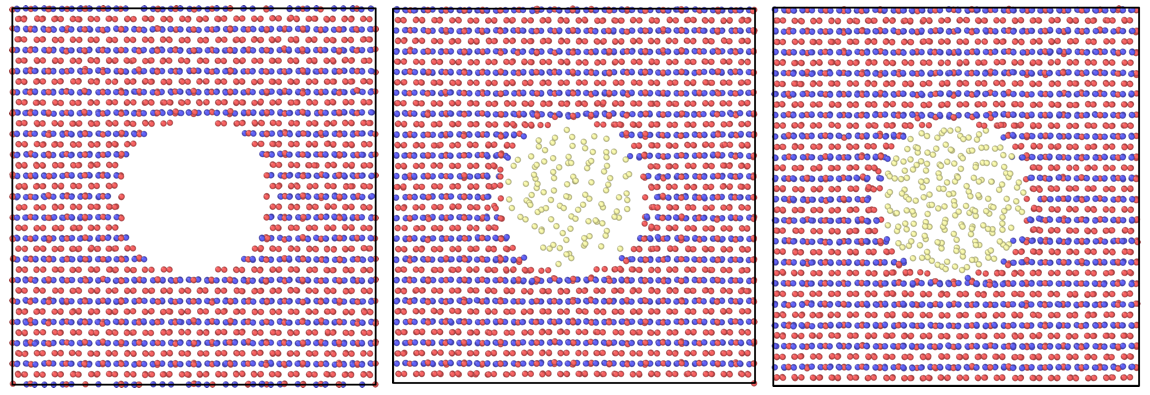
\includegraphics[width=0.9\textwidth]{bub_ex4.png}
 \caption{A Xe bubble in U$_3$Si$_2$. The red atoms are U, blue atoms are Si and yellow atoms are Xe. The Xe/vac ratio is 0, 0.18, and 0.36 moving from left to right. The bubble radius is 16 {\AA} and the system is equilibrated at 400 K.}\label{fig:bub}
\end{figure}

The equation of state can be determined by tracking the pressure inside the bubble and the bubble size as a function of the number of Xe atoms present in the bubble while the system is equilibrated. This provides a pressure versus density relationship which can be fit to an appropriate equation of state. The bubble size is tracked periodically throughout the simulation by calculating the distance between two U atoms on opposite sides of the bubble. The bubble pressure is determined by computing the stress per atom on each Xe atom, summing the individual stress components and subsequently converting to a pressure, as outlined in the LAMMPS dcoumentation \cite{plimpton1995}. Data is gathered at 400 K, 600 K, 800 K and 1000 K and jointly fit to an equation of state (EOS). The EOS for Xe bubbles is taken from Kaplun \cite{kaplun2003}, 

\begin{equation}
\label{eq:EOS}
P=\frac{RT}{v}\bigg( 1+\frac{c}{v-b}\bigg)-\frac{a}{v^2}
\end{equation}

where R is the gas constant for Xe (8.314 J/mol-K\cite{kaplun2003}), T is the temperature in K, P is the pressure in MPa, v is the molar volume in cm$^3$/mol, and a, b, and c are fitting parameters. This EOS reduces to the well known Van der Waals EOS when b=c. The parameters from Kaplun \cite{kaplun2003} for a pure Xe gas are utilized as the starting guess for the fitting procedure in this work to obtain an optimized EOS. A minimization script is utilized to fit the EOS to the determined pressure and molar volume data from the molecular dynamics simulations. The pressure versus volume and temperature data is input into the script, and the squared error is summed and utilized to optimize the EOS, iterating by providing a random step to each of the a, b and c coefficients and only accepting the iteration if the summed error is reduced. A total of 455 data points are utilized in the fitting. 

The optimized parameters are provided in table \ref{tab:eos}, compared to the original parameters from Kaplun \cite{kaplun2003}. Additionally, the molecular dynamics data for the Xe MEAM potential verification presented earlier was fit to an EOS and that fit is provided here for comparison as well. It should be noted that the data in Kaplun was only for low pressure Xe gas (0-50 MPa) and low temperatures (170-500K). This work spans a much higher temperature and pressure regime. 

The optimized EOS for Xe bubbles in U$_3$Si$_2$ is shown in Fig. \ref{fig:eos_sum} for isotherms at 400 K, 600 K, 800 K and 1000 K, compared to molecular dynamics data. The EOS for Xe bubbles fits the molecular dynamics data quite well. Excellent agreement is observed for low pressure systems, with some deviation occurring at high pressures (above 1.5 GPa). The RMSD of the fitted EOS compared to the MEAM data is 156 MPa with a NRMSD of 6.2\%, computed as outlined previously in this manuscript. 

\begin{table}[h]
\caption{The optimized parameters for a Xe EOS in U$_3$Si$_2$. Parameters are shown for Xe bubbles, pure Xe and a previous fit \cite{kaplun2003}.}\label{tab:eos}
\begin{center}
\begin{tabular}{|c|c|c|c|}
 \hline
  & a (J-cm$^3$/mol$^2$) & b (cm$^3$/mol) & c (cm$^3$/mol) \\ 
 \hline
 Xe bubbles & 40000 & 12.0 & 242.9 \\ 
 Xe MEAM & 356591 & 19.3 & 126.5 \\ 
 Kaplun \cite{kaplun2003} & 434242 & 33.8 & 65.6 \\ 
 \hline
\end{tabular}
\end{center}
\label{default}
\end{table}%


\begin{figure}[hbt]
	\centering
	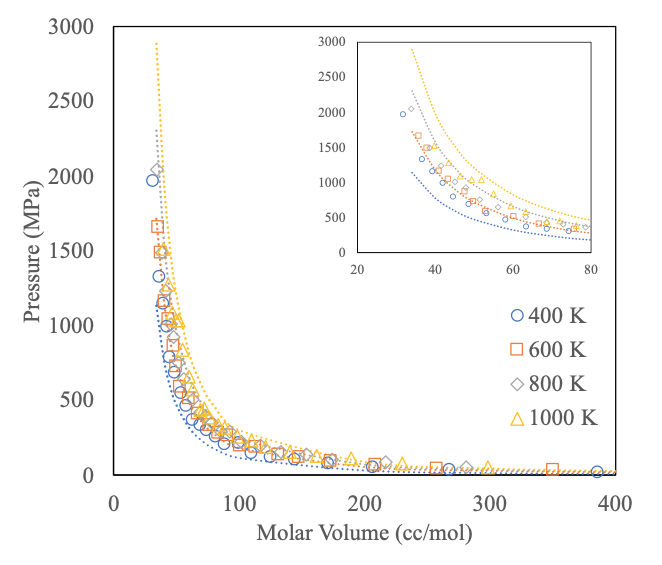
\includegraphics[width=0.8\textwidth]{bubble_eosa.png}
 \caption{Pressure as a function of specific volume for a Xe gas bubble in U$_3$Si$_2$ at 400 K, 600 K, 800 K and 1000 K. Data marked by symbols is molecular dynamics data and dashed lines represent the EOS fit at each of the respective temperatures\DIFaddbeginFL \DIFaddFL{. An inset is included for high pressure/density data}\DIFaddendFL . }\label{fig:eos_sum}
\end{figure}

\FloatBarrier

Generally, the EOS looks quite similar to that from Xe gas in Fig. \ref{fig:xe_eos}, and thus a comparison is warranted to extract information regarding the behavior of Xe in bubbles, compared to pure Xe gas. The comparison of the Xe EOS in bubbles to the pure Xe EOS is shown in Fig. \ref{fig:eos_comp}. It is found that Xe in bubbles exhibits a generally higher pressure than Xe in pure gas over the entire range of molar volumes and temperatures investigated. As the molar volume decreases, the difference in the predicted pressure becomes greater. As the molar volume increases, the data converges, which is essence shows that in very large or low density bubbles, Xe behaves as a pure Xe gas. Comparing the data for Xe bubbles to Xe gas yields a discrepancy with a NRMSD of 14.5\%. This is a non-negligible difference that illustrates the importance of developing a materials-specific EOS for fission gas in bubbles. This EOS can be implemented into mesoscale models to study bubble evolution. The applicable range of this current EOS is much greater than the previous reported EOS by Kaplun \cite{kaplun2003}, whereas this EOS was fit to data from 400 K to 1000 K, and can accurately describe bubbles with pressures from a few MPa up to 2.5 GPa.

\begin{figure}[hbt]
	\centering
	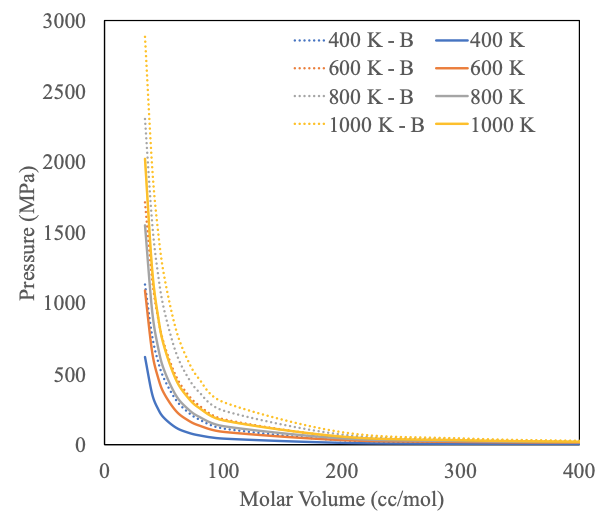
\includegraphics[width=0.8\textwidth]{xe_eos_compa.png}
 \caption{Comparison of the EOS for pure Xe from the MEAM potential to Xe in bubbles (denoted with a - B) in U$_3$Si$_2$.}\label{fig:eos_comp}
\end{figure}

\FloatBarrier

\section{Conclusion}

A modified Embedded-Atom Method interatomic potential was developed for the U-Si-Xe system. Utilizing available potentials from the literature for U \cite{moore2015}, Si and U-Si \cite{beelerusi} and Xe \cite{beelerASTM}, descriptions for U-Xe and Si-Xe were developed by fitting to DFT data. This is the first potential capable of describing this ternary system. This potential performs adequately in describing point defect properties of Xe in U$_3$Si$_2$, does a reasonable job of predicting theoretical intermetallic structures of both UXe and SiXe phases, and performs excellently in matching pressure versus volume experimental data for Xe gas. This potential was then applied to the study of Xe point defect segregation at grain boundaries, showing that higher energy grain boundaries exhibit a stronger segregation energy for Xe defects. Additionally, it was shown that for all grain boundary orientations analyzed, the interaction between grain boundaries and Xe defects is very short range, in that once a defect is beyond 5 {\AA} from the grain boundary, there is not an observable energetic difference from that defect residing in the bulk. Finally an equation of state was developed for Xe bubbles in U$_3$Si$_2$ that can describe systems from 400 K up to 1000 K and pressures up to 2.5 GPa. It was found that the behavior of Xe in bubbles is distinct from a pure Xe gas, and requires a unique EOS. This information can be directly incorporated into mesoscale models to more accurately simulate bubble evolution under reactor operation. 

The development of this ternary interatomic potential provides a tool for further examination of Xe in the U-Si system and a means for fundamental investigations of fission gas behavior that were previously unable to be performed. 


\section{Acknowledgments}
This work is supported by the U.S. Department of Energy, Office of Nuclear Energy, Nuclear Energy Advanced Modeling and Simulation (NEAMS) Program. This work is also supported by U.S. Department of Energy, Office of Nuclear Energy, Nuclear Energy University Partnerships, under contract no. DE-NE0008564. This manuscript has been authored by Battelle Energy Alliance, LLC under Contract No. DEAC07-05ID14517 with the U.S. Department of Energy. The United States Government retains and the publisher, by accepting the article for publication, acknowledges that the United States Government retains a nonexclusive, paid-up, irrevocable, world-wide license to publish or reproduce the published form of this manuscript, or allow others to do so, for United States Government purposes. Los Alamos National Laboratory, an affirmative action/equal opportunity employer, is operated by Los Alamos National Security, LLC, for the National Nuclear Security Administration of the U.S. Department of Energy under Contract No. DE-AC52-06NA25396. This research made use of the resources of the High Performance Computing Center at Idaho National Laboratory, which is supported by the Office of Nuclear Energy of the U.S. Department of Energy and the Nuclear Science User Facilities under Contract No. DE-AC07-05ID14517.


\bibliography{MARMOTbib.bib}

\end{document}




